% https://en.wikipedia.org/wiki/Cut_(graph_theory)
\section{Puentes}\label{bridges}
Una arista se llama puente si al eliminarla del grafo (manteniendo los vértices) aumenta el número de componentes conectados \cite{Jaimini2017}.

\begin{figure}[H]
	\centering
	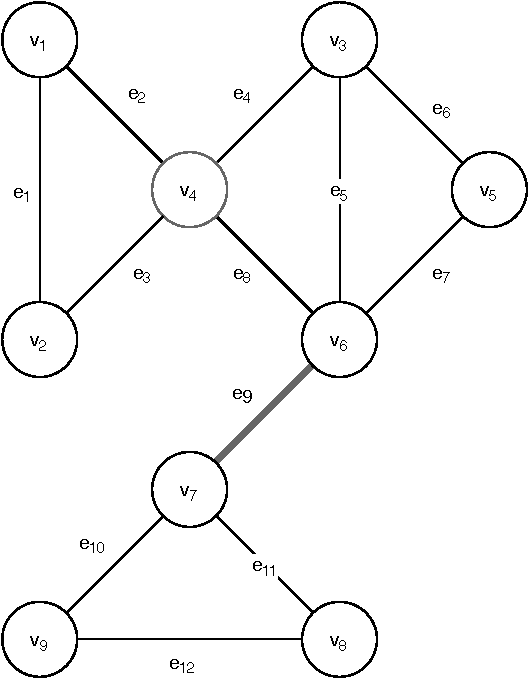
\includegraphics[width=0.4\linewidth]{document/ArticulationPoints/images/example-of-bridge}
	\caption{Ejemplo de grafo con una arista puente \( e_9 \).}
	\label{fig:example-of-bridge}
\end{figure}

\section{Trabajo futuro}\label{futurework}
Como continuación de este trabajo, se presentan problemas propuestos en \textit{UVa Online Judge} relacionados a la categoría de puntos de articulación. Se propone la siguiente colección de problemas:
\begin{itemize}
	\item UVa 315 - Network
	\item UVa 610 - Street Directions
	\item UVa 796 - Critical Links
	\item UVa 10199 - Tourist Guide
	\item UVa 10765 - Doves and bombs
\end{itemize}